\section{Auswertung}
Die in der Auswertung bestimmten Ausgleichsrechnungen werden mit
dem Python Paket \emph{scipy.optimize}\cite{scipy} durchgeführt. Zur Analyse der aufgenommen Fotos
wird das Paket \emph{scipy.misc}\cite{scipy} verwendet. Dieses ermöglicht jedem Pixel der Fotos einen
Wert in Abhängigkeit von der Helligkeit zuzuordnen. Dieser Wert ist quantitativ irrelevant für die
Auswertung des Versuches, da lediglich die Lage der Intensitätsmaxima bestimmt werden soll. Hierzu wird
jeweils exakt in der Mitte der Bilder eine Reihe aus den eingelesenen Pixeln entnommen und die Helligkeit
in Abhängigkeit von der horizontalen Lage graphisch dargestellt.  
\subsection{Aufnahme der Hysterese}
Die gemessenen magnetischen Flussdichten $B$ in Abhängigkeit der angelegten Stromstärke $I$
sind in Tabelle \ref{tab: hysterese} aufgetragen. Eine graphische Darstellung befindet sich in Abbildung
\ref{fig: hysterese_gesamt}. Mittels der Messwerte wird eine Regression nach dem Prinzip der kleinsten Quadrate
an eine Funktion der Form
\begin{equation}
  B(I) = a_1 I^3 + a_2 I^2 + a_3 I ^2 + a_4
  \label{eq: fitfuntion_hysterese}
\end{equation}
bestimmt. Für den austeigenden Ast der Hysterese ergeben sich folgende Parameter
\begin{align}
  \begin{aligned}
    a_1 &= \SI{-0.7(1)e-1}{\milli\tesla \per \ampere ^3} & a_2 &= \SI{1.5(3)}{\milli\tesla \per \ampere ^2} \\
    a_3 &= \SI{5.1(3)e1}{\milli\tesla \per \ampere } & a_4 &= \SI{3(6)}{\milli\tesla }.
    \label{eq: params_up}
  \end{aligned}
\end{align}
Analog werden folgende Werte für den absteigenden Ast gefunden
\begin{align}
  \begin{aligned}
    b_1 &= \SI{-8.6(8)e-2}{\milli\tesla \per \ampere ^3} & b_2 &= \SI{1.9(3)}{\milli\tesla \per \ampere ^2} \\
    b_3 &= \SI{4.7(2)e1}{\milli\tesla \per \ampere } & b_4 &= \SI{11(4)}{\milli\tesla }.
  \end{aligned}
\end{align}
Eine graphische Darstellung der Fitfunktionen befindet sich in Abbildung \ref{fig: hysterese_fit}.
\subsection{Aufnahme der Hysterese}
Die gemessenen magnetischen Flussdichten $B$ in Abhängigkeit der angelegten Stromstärke $I$
sind in Tabelle \ref{tab: hysterese} aufgetragen. Eine graphische Darstellung befindet sich in Abbildung
\ref{fig: hysterese_gesamt}. Mittels der Messwerte wird eine Regression nach dem Prinzip der kleinsten Quadrate
an eine Funktion der Form
\begin{equation}
  B(I) = a_1 I^3 + a_2 I^2 + a_3 I ^2 + a_4
  \label{eq: fitfuntion_hysterese}
\end{equation}
bestimmt. Für den austeigenden Ast der Hysterese ergeben sich folgende Parameter
\begin{align}
  \begin{aligned}
    a_1 &= \SI{-0.7(1)e-1}{\milli\tesla \per \ampere ^3} & a_2 &= \SI{1.5(3)}{\milli\tesla \per \ampere ^2} \\
    a_3 &= \SI{5.1(3)e1}{\milli\tesla \per \ampere } & a_4 &= \SI{3(6)}{\milli\tesla }.
    \label{eq: params_up}
  \end{aligned}
\end{align}
Analog werden folgende Werte für den absteigenden Ast gefunden
\begin{align}
  \begin{aligned}
    b_1 &= \SI{-8.6(8)e-2}{\milli\tesla \per \ampere ^3} & b_2 &= \SI{1.9(3)}{\milli\tesla \per \ampere ^2} \\
    b_3 &= \SI{4.7(2)e1}{\milli\tesla \per \ampere } & b_4 &= \SI{11(4)}{\milli\tesla }.
  \end{aligned}
\end{align}
Eine graphische Darstellung der Fitfunktionen befindet sich in Abbildung \ref{fig: hysterese_fit}.
\subsection{Aufnahme der Hysterese}
Die gemessenen magnetischen Flussdichten $B$ in Abhängigkeit der angelegten Stromstärke $I$
sind in Tabelle \ref{tab: hysterese} aufgetragen. Eine graphische Darstellung befindet sich in Abbildung
\ref{fig: hysterese_gesamt}. Mittels der Messwerte wird eine Regression nach dem Prinzip der kleinsten Quadrate
an eine Funktion der Form
\begin{equation}
  B(I) = a_1 I^3 + a_2 I^2 + a_3 I ^2 + a_4
  \label{eq: fitfuntion_hysterese}
\end{equation}
bestimmt. Für den austeigenden Ast der Hysterese ergeben sich folgende Parameter
\begin{align}
  \begin{aligned}
    a_1 &= \SI{-0.7(1)e-1}{\milli\tesla \per \ampere ^3} & a_2 &= \SI{1.5(3)}{\milli\tesla \per \ampere ^2} \\
    a_3 &= \SI{5.1(3)e1}{\milli\tesla \per \ampere } & a_4 &= \SI{3(6)}{\milli\tesla }.
    \label{eq: params_up}
  \end{aligned}
\end{align}
Analog werden folgende Werte für den absteigenden Ast gefunden
\begin{align}
  \begin{aligned}
    b_1 &= \SI{-8.6(8)e-2}{\milli\tesla \per \ampere ^3} & b_2 &= \SI{1.9(3)}{\milli\tesla \per \ampere ^2} \\
    b_3 &= \SI{4.7(2)e1}{\milli\tesla \per \ampere } & b_4 &= \SI{11(4)}{\milli\tesla }.
  \end{aligned}
\end{align}
Eine graphische Darstellung der Fitfunktionen befindet sich in Abbildung \ref{fig: hysterese_fit}.
\input{../Messdaten/tabs/hysterese.tex}
\begin{figure}
  \centering
  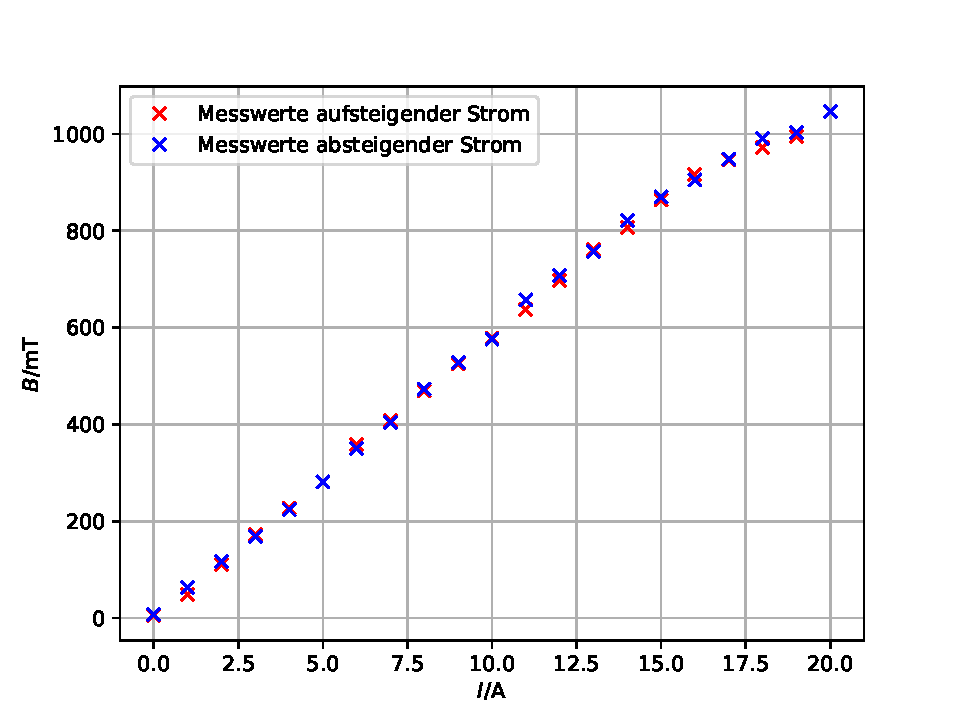
\includegraphics[width = \textwidth]{../Messdaten/plots/hysterese_data.pdf}
  \caption{Graphische Darstellung der Messwerte zur Bestimmung des Zusammenhangs $B(I)$ zwischen angelegtem Strom $I$ und
  magnetischer Flussdichte $B$ des Elektromagneten.}
  \label{fig: hysterese_gesamt}
\end{figure}
\begin{figure}
  \centering
  \begin{subfigure}{0.48\textwidth}
    \centering
  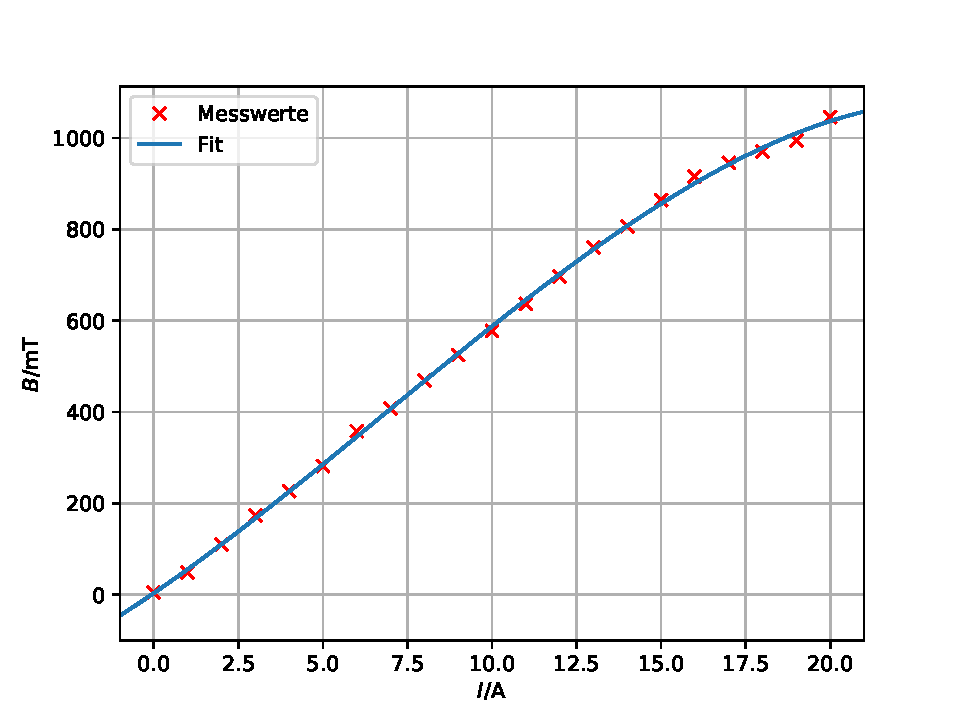
\includegraphics[width = \textwidth]{../Messdaten/plots/hysterese_aufsteigend.pdf}
  \caption{Aufsteigender Strom $I$.}
  \label{fig: hysterese_aufsteigend}
\end{subfigure}
\hfill
  \begin{subfigure}{0.48\textwidth}
  \centering
  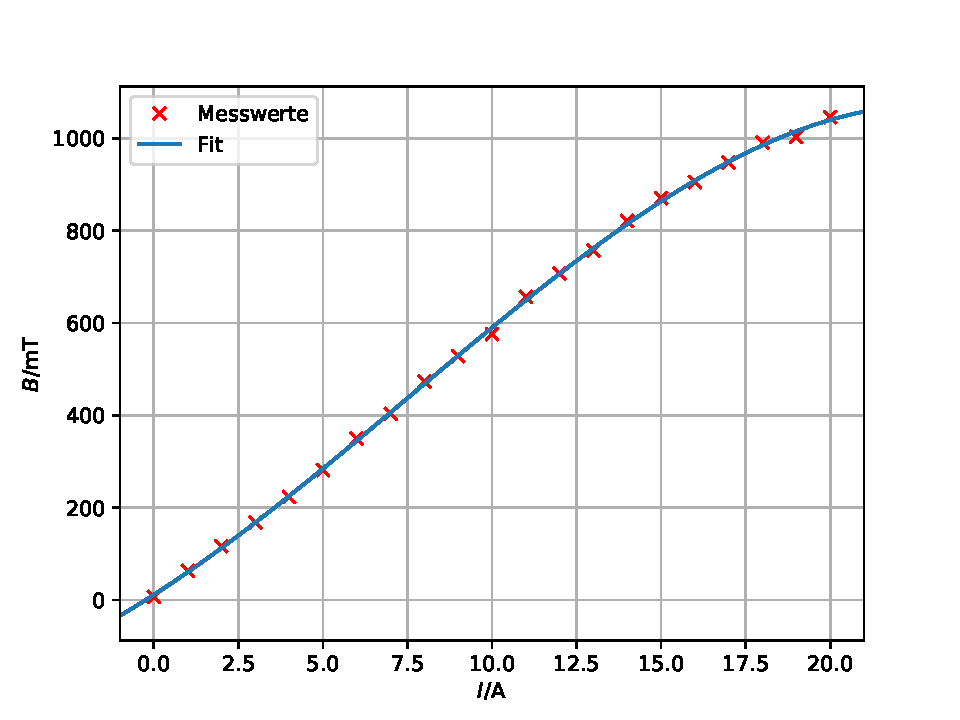
\includegraphics[width = \textwidth]{../Messdaten/plots/hysterese_absteigend.pdf}
  \caption{Absteigender Strom $I$.}
  \label{fig: hysterese_absteigend}
\end{subfigure}
\caption{Graphische Darstellung der Abhängigkeit $B(I)$ unter ab-/aufsteigendem Strom $I$ mit jeweiliger Regressionskurve.}
\label{fig: hysterese_fit}
\end{figure}
Im Folgenden wird Gleichung \eqref{eq: fitfuntion_hysterese} mit den Parametern \eqref{eq: params_up}
verwendet um den notwendigen Zusammenhang zwischen angelegtem Strom $I$ und magnetischer Flussdichte $B$ herzustellen.

\begin{figure}
  \centering
  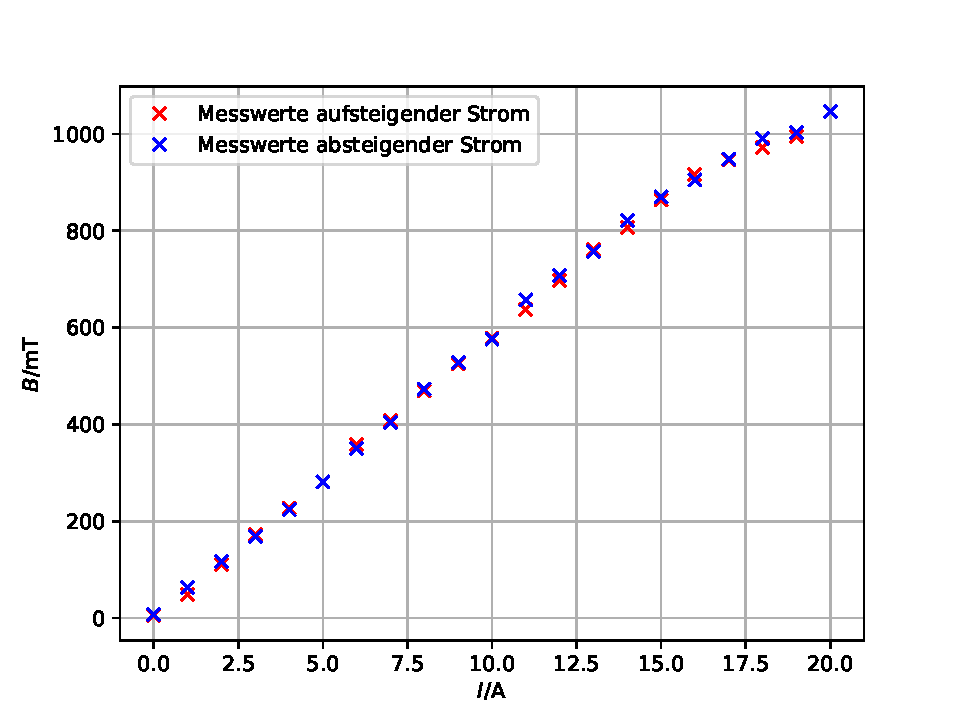
\includegraphics[width = \textwidth]{../Messdaten/plots/hysterese_data.pdf}
  \caption{Graphische Darstellung der Messwerte zur Bestimmung des Zusammenhangs $B(I)$ zwischen angelegtem Strom $I$ und
  magnetischer Flussdichte $B$ des Elektromagneten.}
  \label{fig: hysterese_gesamt}
\end{figure}
\begin{figure}
  \centering
  \begin{subfigure}{0.48\textwidth}
    \centering
  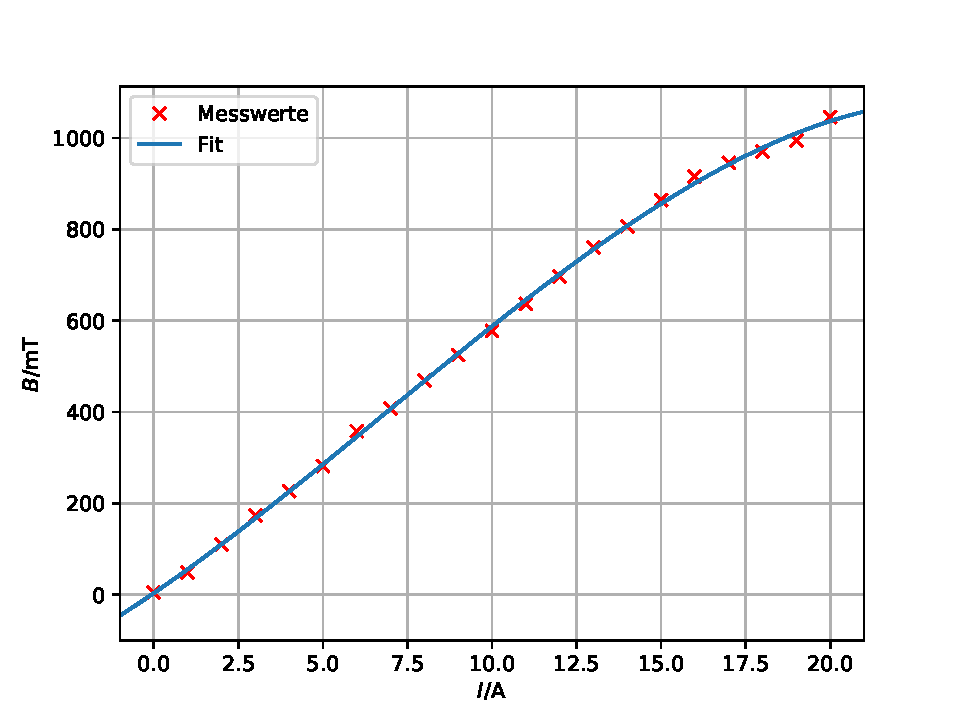
\includegraphics[width = \textwidth]{../Messdaten/plots/hysterese_aufsteigend.pdf}
  \caption{Aufsteigender Strom $I$.}
  \label{fig: hysterese_aufsteigend}
\end{subfigure}
\hfill
  \begin{subfigure}{0.48\textwidth}
  \centering
  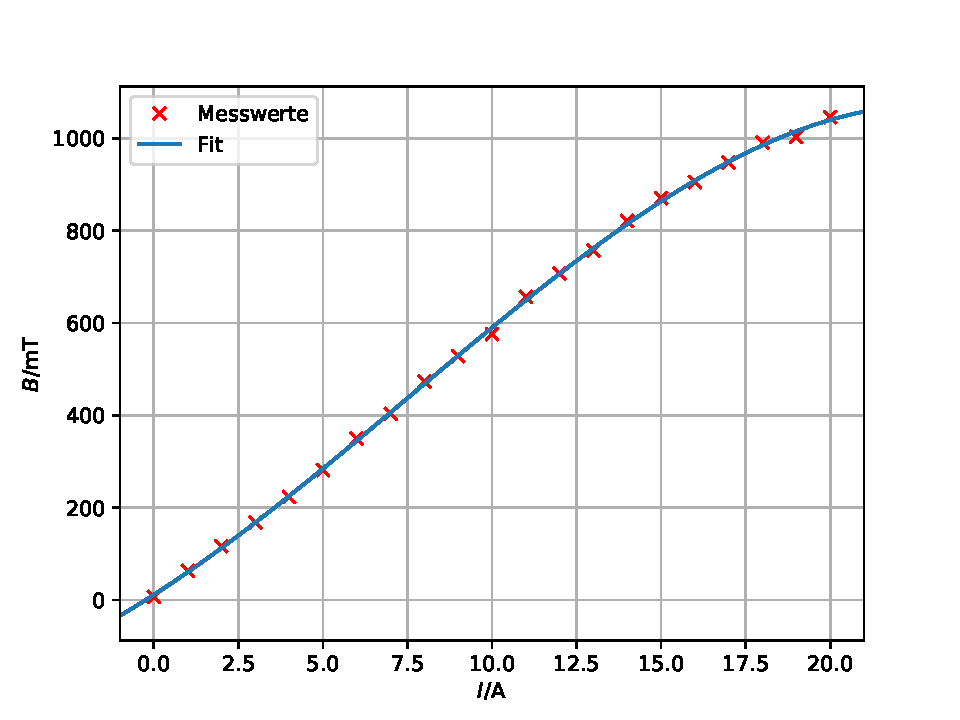
\includegraphics[width = \textwidth]{../Messdaten/plots/hysterese_absteigend.pdf}
  \caption{Absteigender Strom $I$.}
  \label{fig: hysterese_absteigend}
\end{subfigure}
\caption{Graphische Darstellung der Abhängigkeit $B(I)$ unter ab-/aufsteigendem Strom $I$ mit jeweiliger Regressionskurve.}
\label{fig: hysterese_fit}
\end{figure}
Im Folgenden wird Gleichung \eqref{eq: fitfuntion_hysterese} mit den Parametern \eqref{eq: params_up}
verwendet um den notwendigen Zusammenhang zwischen angelegtem Strom $I$ und magnetischer Flussdichte $B$ herzustellen.

\begin{figure}
  \centering
  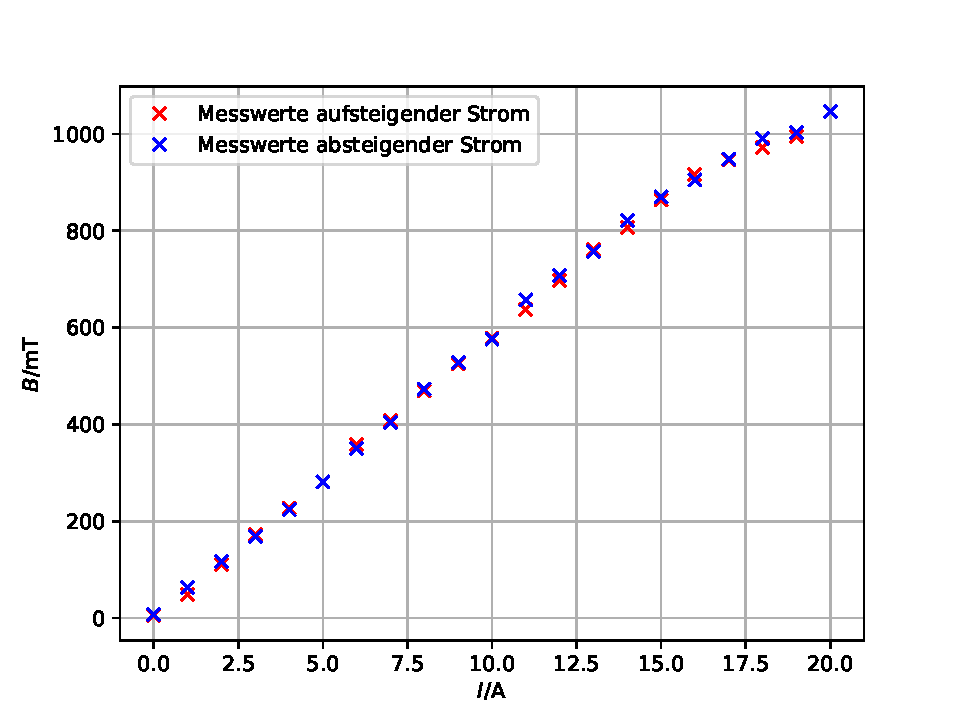
\includegraphics[width = \textwidth]{../Messdaten/plots/hysterese_data.pdf}
  \caption{Graphische Darstellung der Messwerte zur Bestimmung des Zusammenhangs $B(I)$ zwischen angelegtem Strom $I$ und
  magnetischer Flussdichte $B$ des Elektromagneten.}
  \label{fig: hysterese_gesamt}
\end{figure}
\begin{figure}
  \centering
  \begin{subfigure}{0.48\textwidth}
    \centering
  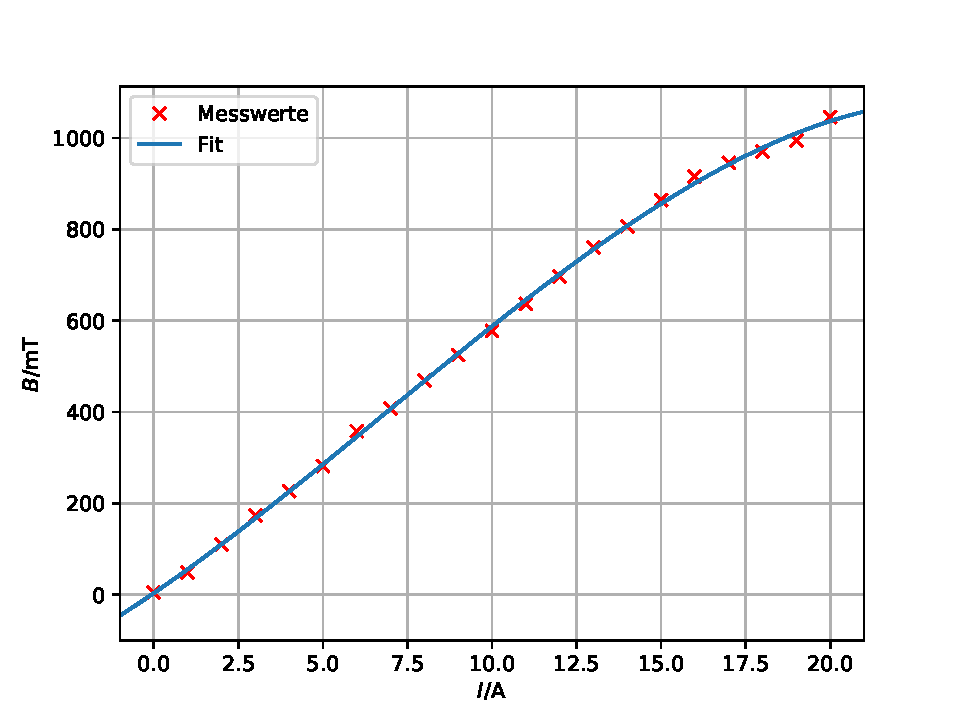
\includegraphics[width = \textwidth]{../Messdaten/plots/hysterese_aufsteigend.pdf}
  \caption{Aufsteigender Strom $I$.}
  \label{fig: hysterese_aufsteigend}
\end{subfigure}
\hfill
  \begin{subfigure}{0.48\textwidth}
  \centering
  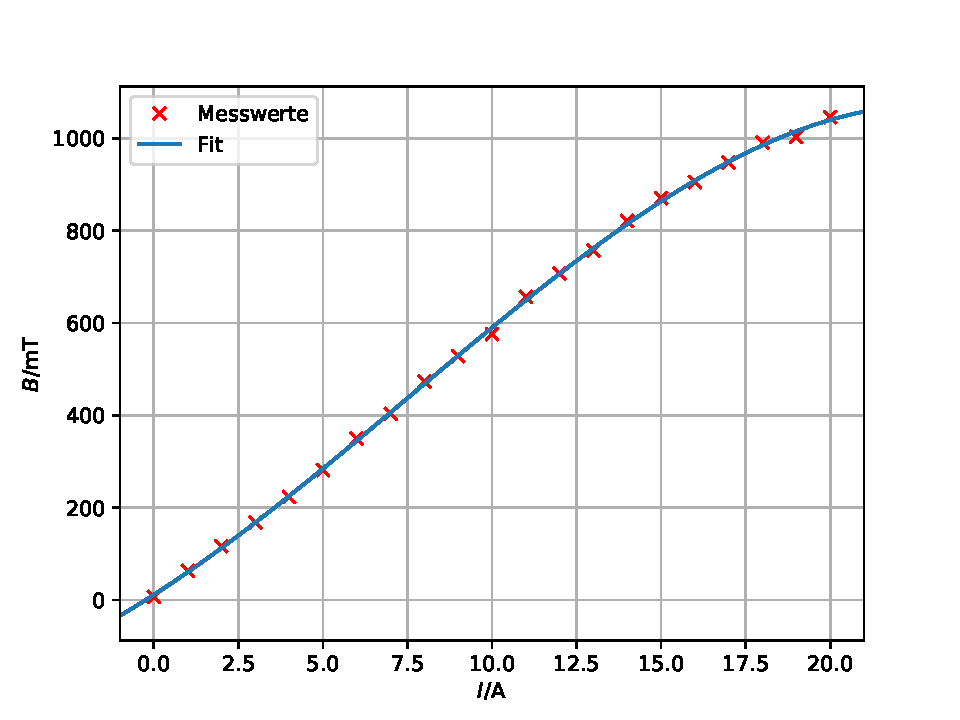
\includegraphics[width = \textwidth]{../Messdaten/plots/hysterese_absteigend.pdf}
  \caption{Absteigender Strom $I$.}
  \label{fig: hysterese_absteigend}
\end{subfigure}
\caption{Graphische Darstellung der Abhängigkeit $B(I)$ unter ab-/aufsteigendem Strom $I$ mit jeweiliger Regressionskurve.}
\label{fig: hysterese_fit}
\end{figure}
Im Folgenden wird Gleichung \eqref{eq: fitfuntion_hysterese} mit den Parametern \eqref{eq: params_up}
verwendet um den notwendigen Zusammenhang zwischen angelegtem Strom $I$ und magnetischer Flussdichte $B$ herzustellen.

\FloatBarrier
\subsection{Analyse der roten $\sigma$-Linien}
Die Aufspaltung der roten Spektrallinie ist in \autoref{fig: aufspaltung_rot} dargestellt. Zur quantitativen Analyse der Auspaltung wird das
Resultat unter anliegendem Strom von $I = \SI{10}{\ampere}$ verwendet. Gemäß Formel~\eqref{eq: fitfuntion_hysterese} bedingt dieser
eine magnetische Flussdichte von $B = \SI{587(3)}{\milli\tesla}$.

Die Helligkeit in Abhängigkeit von der horizontalen Position auf den aufgenommenen Bilder ist in \autoref{fig: rot_intensität} für das unaufgespaltene
und aufgespaltene Beugungsbild dargestellt. Anhand dessen werden die Positionen von $12$ Intensitätsmaxima und ihrer Aufspaltungen
vermessen. Die Daten sind in \autoref{tab: peaks_rot} aufgeführt. Eine graphische Darstellung der abgelesenen Intensitätsmaxima befindet sich in
den Abbildungen~\ref{fig: peaks_rot_0} und~\ref{fig: peaks_rot_10}.

Die für die Berechnung der Wellenlängenänderung relevanten Abstände $\symup{\Delta} s_i$ und $\symup{\Delta} s_i$ sind in \autoref{tab: abstände_rot}
aufgeführt. Mit Hilfe der Gleichungen~\eqref{} berechnen sich hieraus die Wellenlängenaufspaltung $\symup{\Delta} \lambda$, die
Energieaufspaltung $\symup{\Delta} E$ und schließlich die Werte für die Übergangs-Landé-Faktoren $g$. Alle Ergebnisse sind ebenfalls in
\autoref{tab: abstände_rot} eingetragen. Als Mittelwert für den Landé-Faktor ergibt sich
\begin{equation}
  g_{ij} = \num{1.045(5)}.
\end{equation}
\begin{figure}
  \centering
  \includegraphics[width = 0.7\textwidth]{../Messdaten/bilder_v27/messung_1_rot_sigma/aufspaltung_rot.png}
  \caption{Aufgenommene Intensitätsstreifen des roten Lichtes unter (von oben nach unten) $\SI{0}{\ampere}$, $\SI{7.5}{\ampere}$ und $\SI{10}{\ampere}$.}
  \label{fig: aufspaltung_rot}
\end{figure}
\begin{figure}
  \centering
  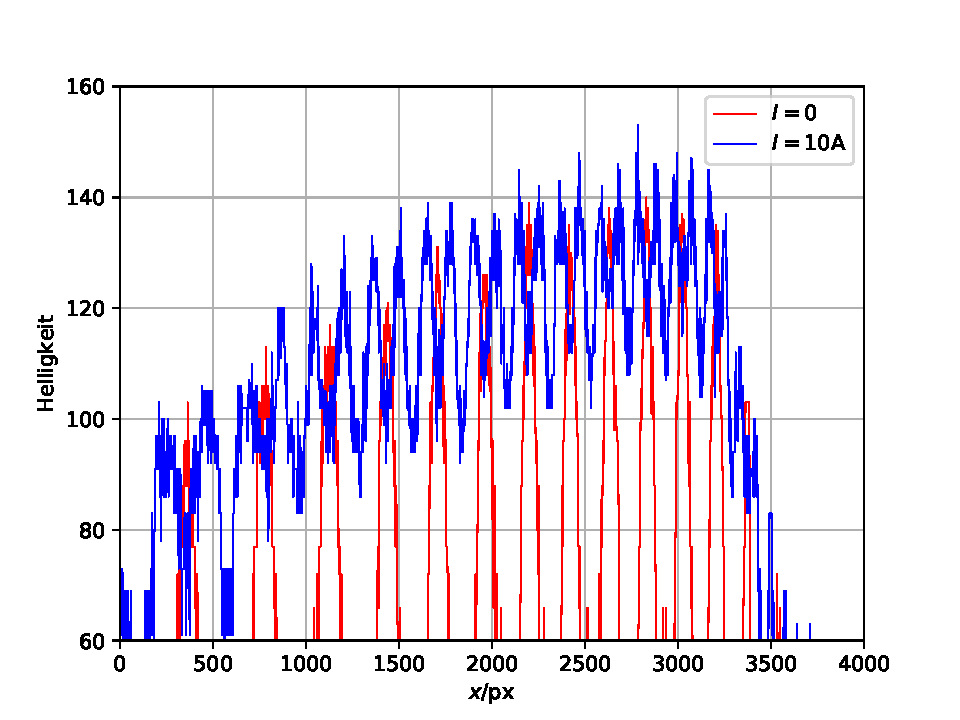
\includegraphics[width = 0.7\textwidth]{../Messdaten/plots/rot_sigma_intensitaet.pdf}
  \caption{Darstellung der Helligkeit der roten Linien in Abhängigkeit von der horizontalen Lage auf dem Foto.}
  \label{fig: rot_intensität}
\end{figure}
\begin{table}
\centering
\caption{Positionen $x_0$ und $x_{10}$ der Intensitätsmaxima unter $I= \SI{0}{\ampere}$ und $I= \SI{10}{\ampere}$.}
\label{tab: peaks_rot}
\begin{tabular}{S S[table-format=4.0] S[table-format=4.0] }
\toprule
{$x_0 /$ px} & \multicolumn{2}{c}{$x_{10} \:/\: $px} \\
\midrule
364 & 234 & 2145\\
784 & 470 & 2254\\
1132 & 693 & 2376\\
1436 & 865 & 2471\\
1705 & 1029 & 2579\\
1964 & 1207 & 2676\\
2201 & 1360 & 2782\\
2415 & 1511 & 2877\\
2632 & 1653 & 2980\\
2830 & 1775 & 3069\\
3022 & 1900 & 3166\\
3205 & 2017 & 3255\\
\bottomrule
\end{tabular}
\end{table}

\begin{figure}
  \centering
  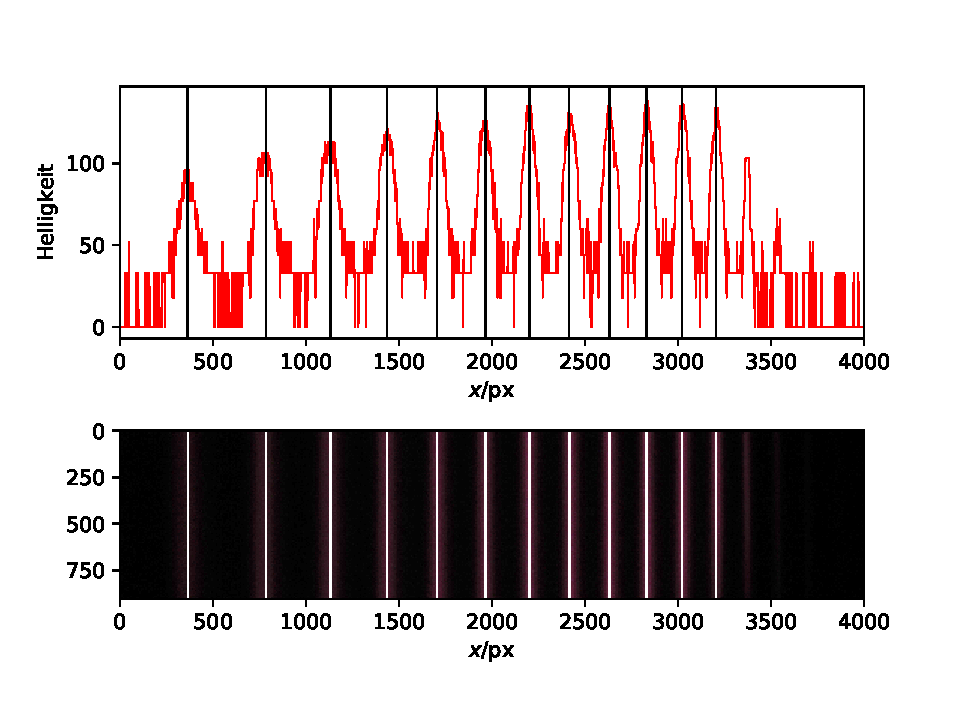
\includegraphics[width = 0.7\textwidth]{../Messdaten/plots/peaks_rot_sigma_0.pdf}
  \caption{Darstellung der abgelesenen Lagen der Intesitätsmaxima für das Beugungsbild unter $I =\SI{0}{\ampere}$.}
  \label{fig: peaks_rot_0}
\end{figure}
\begin{figure}
  \centering
  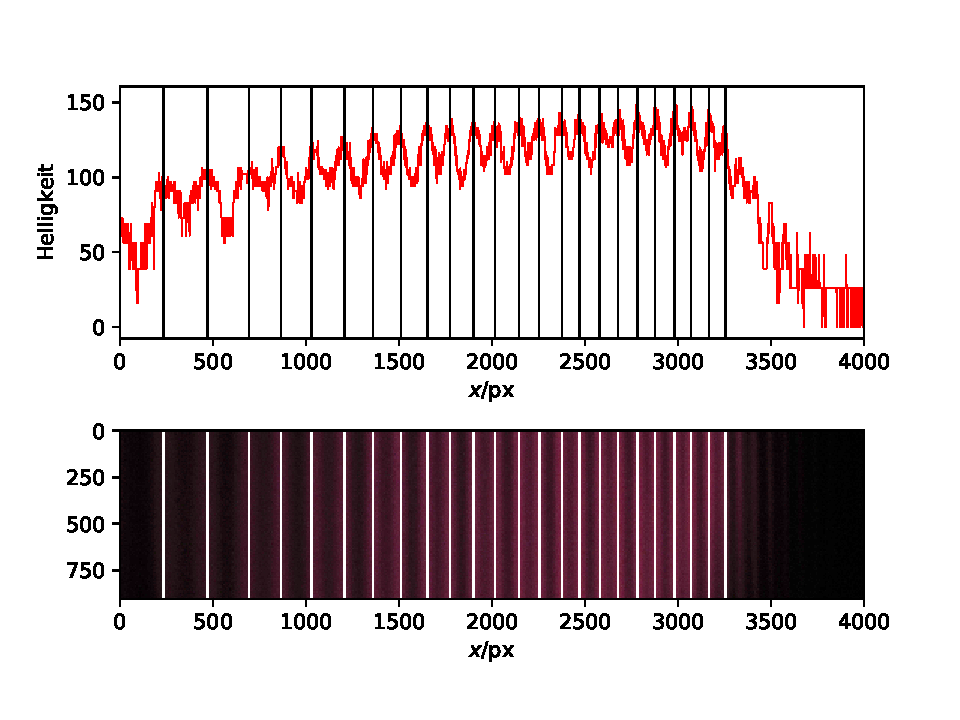
\includegraphics[width = 0.7\textwidth]{../Messdaten/plots/peaks_rot_sigma_10.pdf}
  \caption{Darstellung der abgelesenen Lagen der Intesitätsmaxima für das Beugungsbild unter $I =\SI{10}{\ampere}$.}
  \label{fig: peaks_rot_10}
\end{figure}
\input{../Messdaten/tabs/abstände_rot.tex}

\FloatBarrier
\subsection{Analyse der blauen $\sigma$-Linien}
Die Aufspaltung der blauen Spektrallinie ist in Abbildung \ref{fig: aufspaltung_blau_sigma} dargestellt. Gemäß Formel \eqref{eq: fitfuntion_hysterese}
bedingt dieser eine magnetische Flussdichte von $B = \SI{587(3)}{\milli\tesla}$.
\begin{figure}
  \centering
  \includegraphics[width = 0.7\textwidth]{../Messdaten/bilder_v27/messung_2_blau_sigma/aufspaltung_blau_sigma.png}
  \caption{Sigma Aufspaltung: Aufgenommene Intensitätsstreifen des blauen Lichtes (von oben nach unten) $\SI{0}{\ampere}$ und $\SI{6}{\ampere}$ Spulenstrom.}
  \label{fig: aufspaltung_blau}
\end{figure}
Die Helligkeit in Abhängigkeit von der horizontalen Position auf den aufgenommenen Bilder ist in Abbildung \ref{fig: blau_intensität} für das unaufgespaltene
und aufgespaltene Beugungsbild dargestellt. Anhand dessen werden die Positionen von $12$ Intensitätsmaxima und ihrer Aufspaltungen
vermessen. Die Daten sind in Tabelle \ref{tab: peaks_blau} aufgeführt.
\begin{figure}
  \centering
  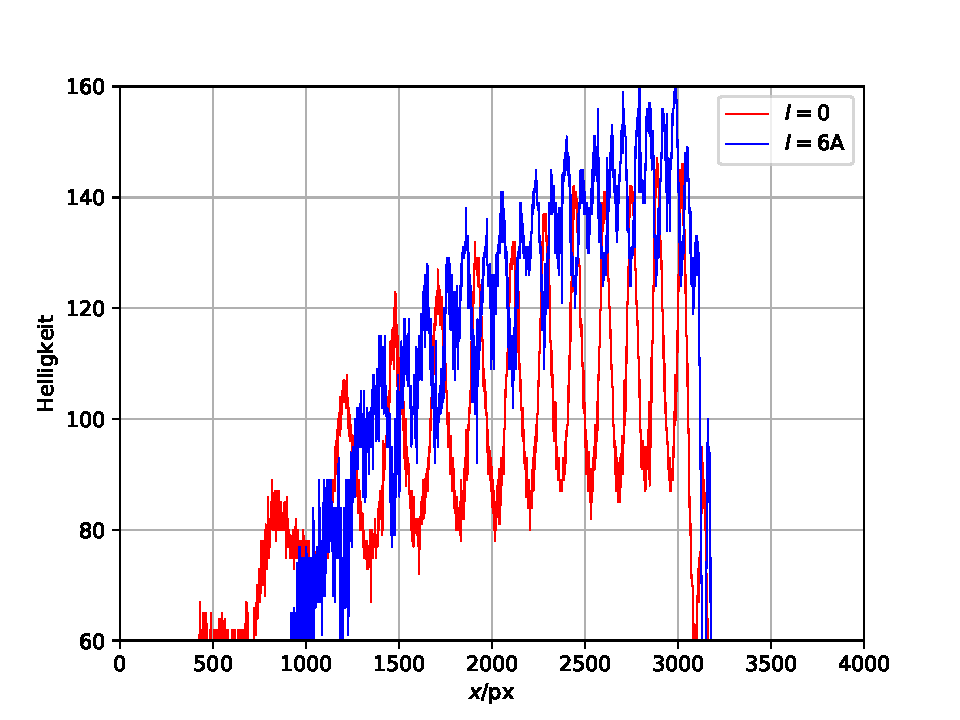
\includegraphics[width = 0.7\textwidth]{../Messdaten/plots/blau_sigma_intensitaet.pdf}
  \caption{Sigma: Darstellung der Helligkeit der blauen Linien in Abhängigkeit von der horizontalen Lage auf dem Foto.}
  \label{fig: blau_intensität_sigma}
\end{figure}
\begin{table}
\centering
\caption{Blaue Sigma Aufspaltung: Positionen $x_0$ und $x_{6}$ der Intensitätsmaxima unter $I= \SI{0}{\ampere}$ und $I= \SI{6}{\ampere}$.}
\label{tab: peaks_blau_sigma}
\begin{tabular}{S S[table-format=4.0] S[table-format=4.0] } 
\toprule
{$x_0 / $px} & \multicolumn{2}{c}{$x_{6} \:/\: $px} \\
\midrule
1483 & 1408 & 2402\\
1708 & 1539 & 2487\\
1909 & 1641 & 2555\\
2121 & 1759 & 2641\\
2285 & 1859 & 2702\\
2449 & 1967 & 2788\\
2605 & 2051 & 2843\\
2752 & 2154 & 2930\\
2891 & 2235 & 2985\\
3030 & 2320 & 3052\\
\bottomrule
\end{tabular}
\end{table}

Eine graphische Darstellung der abgelesenen Intensitätsmaxima befindet sich in den Abbildungen \ref{fig: peaks_blau_0} und \ref{fig: peaks_blau_sigma_6}.
\begin{figure}
  \centering
  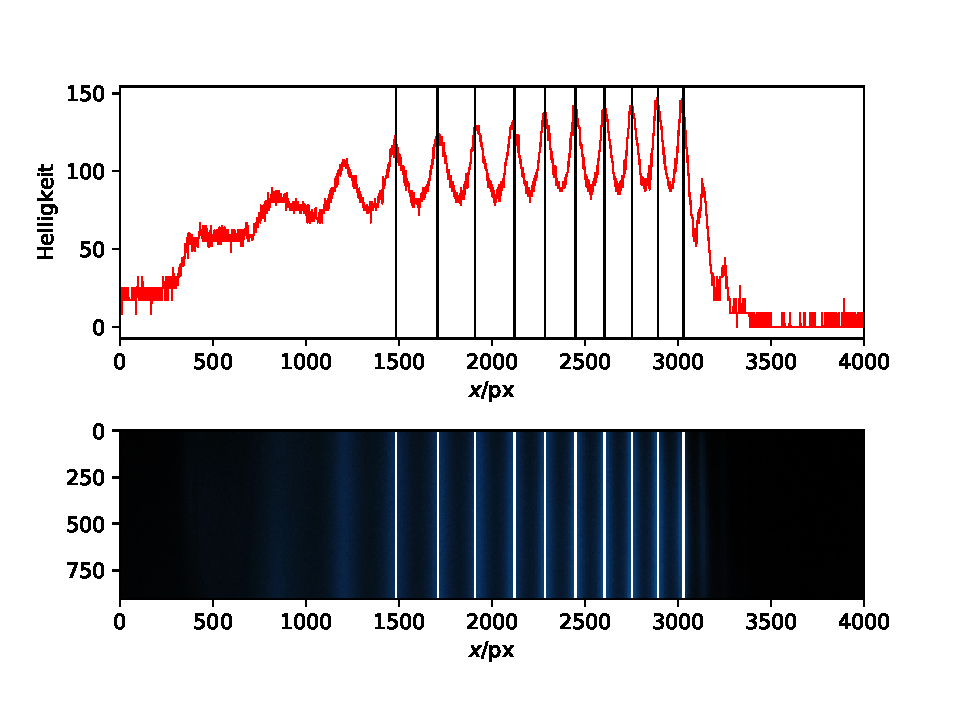
\includegraphics[width = 0.7\textwidth]{../Messdaten/plots/peaks_blau_sigma_0.pdf}
  \caption{Darstellung der abgelesenen Lagen der Intesitätsmaxima für das Beugungsbild unter $I =0$A.}
  \label{fig: peaks_blau_0}
\end{figure}
\begin{figure}
  \centering
  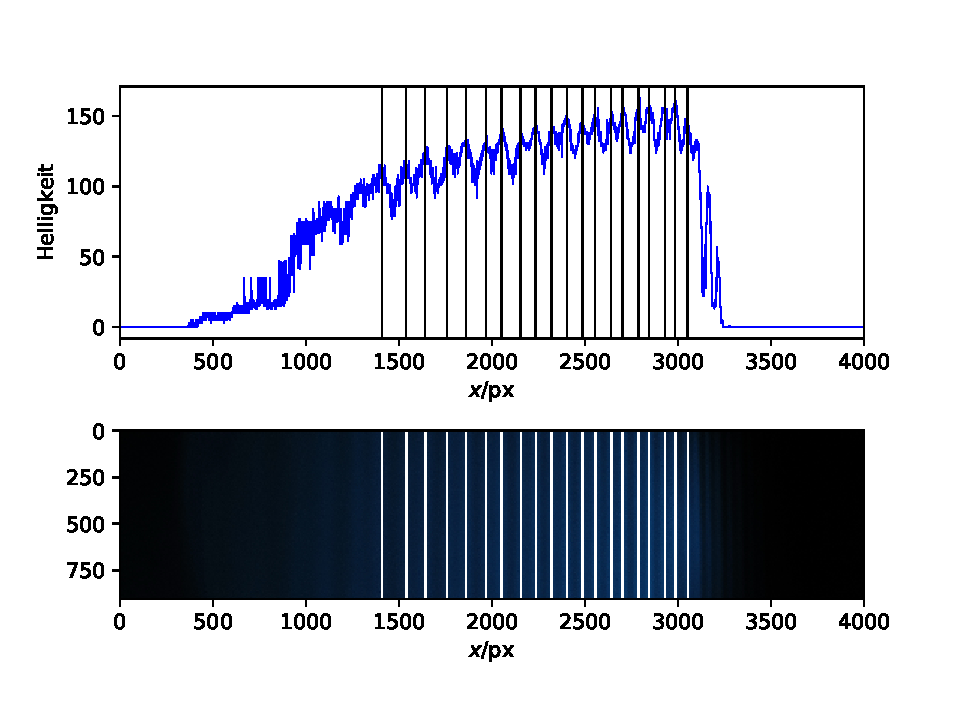
\includegraphics[width = 0.7\textwidth]{../Messdaten/plots/peaks_blau_sigma_6.pdf}
  \caption{Sigma: Darstellung der abgelesenen Lagen der Intesitätsmaxima für das Beugungsbild unter $I =6$A.}
  \label{fig: peaks_blau_sigma_6}
\end{figure}
Die für die Berechnung der Wellenlängenänderung relevanten Abstände $\Delta s_i$ und $\delta s_i$ sind in Tabelle \ref{tab: abstände_blau_sigma}
aufgeführt. Mit Hilfe der Gleichungen \eqref{} berechnen sich hieraus die Wellenlängenaufspaltung $\Delta \lambda$, die
Energieaufspaltung $\Delta E$ und schließlich die Werte für die Übergangs-Landé-Faktoren $g$. Alle Ergebnisse sind ebenfalls in
Tabelle \ref{tab: abstände_blau_sigma} eingetragen. Als Mittelwert für den Lande-Faktor ergibt sich
\begin{equation}
  g = \num{1.045(5)}.
\end{equation}
\input{../Messdaten/tabs/abstände_blau_sigma.tex}

\FloatBarrier
\subsection{Analyse der blauen $\pi$ Linien}
Die Aufspaltung der blauen Spektrallinien ist in \autoref{fig: aufspaltung_blau_pi} einzusehen. Diese wird bei einem
Feldstrom von $I = \SI{17}{\ampere}$ beobachtet, was gemäß~\eqref{eq: fitfuntion_hysterese} auf $B = \SI{942(3)}{\milli\tesla}$ führt.

Die Helligkeit in Abhängigkeit von der horizontalen Position auf den aufgenommenen Bilder ist in \autoref{fig: blau_intensität_pi} für das aufgespaltene Beugungsbild dargestellt.
Anhand dessen werden erneut die Positionen von $10$ Intensitätsmaxima und ihrer Aufspaltungen
vermessen. Die Daten sind in \autoref{tab: peaks_blau_pi} eingetragen. Eine graphische Darstellung
der abgelesenen Intensitätsmaxima befindet sich in den Abbildungen~\ref{fig: peaks_blau_0} und~\ref{fig: peaks_blau_pi_17}.

Die Werte für $\Delta s_i$ und $\delta s_i$ sowie die Ergebnisse der Rechnungen sind in \autoref{tab: abstände_blau_pi} eingetragen.
Als Mittelwert für den Landé-Faktor ergibt sich
\begin{equation}
  g_{ij} = \num{0.581(2)}.
\end{equation}
\begin{figure}
  \centering
  \includegraphics[width = 0.7\textwidth]{../Messdaten/bilder_v27/messung_3_blau_pi/aufspaltung_blau_pi.png}
  \caption{Blau $\pi$: Aufgenommene Intensitätsstreifen des blauen Lichtes (von oben nach unten) $\SI{0}{\ampere}$ und $\SI{17}{\ampere}$ Feldstrom.}
  \label{fig: aufspaltung_blau_pi}
\end{figure}
\begin{figure}
  \centering
  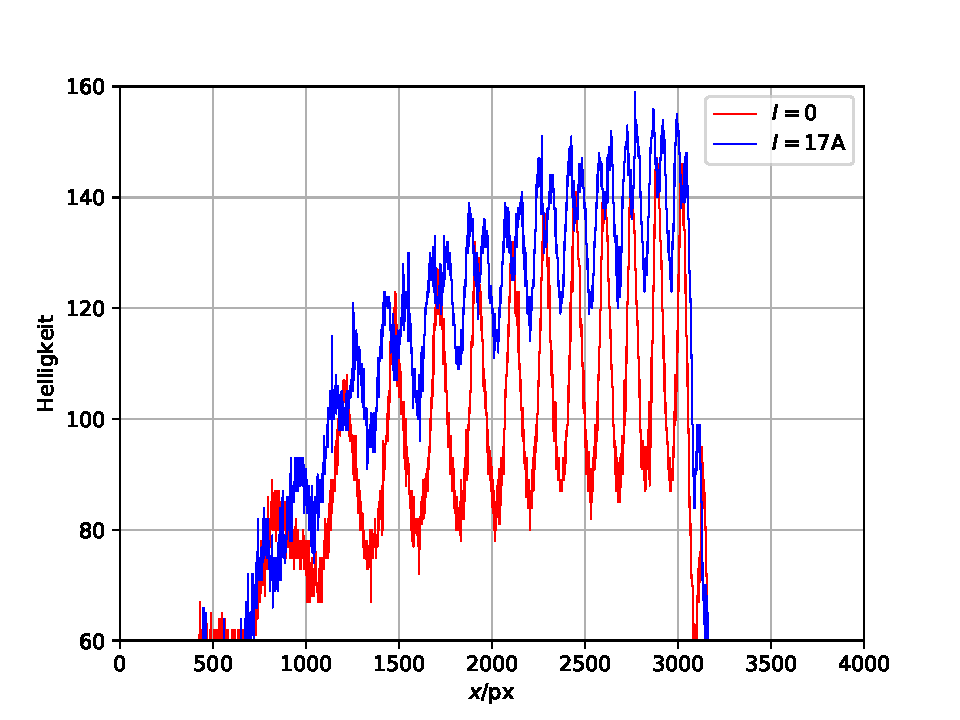
\includegraphics[width = 0.7\textwidth]{../Messdaten/plots/blau_pi_intensitaet.pdf}
  \caption{Blau $\pi$: Darstellung der Helligkeit der blauen Linien in Abhängigkeit von der horizontalen Lage auf dem Foto.}
  \label{fig: blau_intensität_pi}
\end{figure}
\begin{table}
\centering
\caption{Blau $\pi$: Positionen $x_0$ und $x_{17}$ der Intensitätsmaxima unter $I= \SI{0}{\ampere}$ und $I= \SI{17}{\ampere}$.}
\label{tab: peaks_blau_pi}
\begin{tabular}{S S[table-format=4.0]  S[table-format=4.0] } 
\toprule
{$x_0 / $px} & \multicolumn{2}{c}{$x_{17} \:/\: $px} \\
\midrule
1205 & 1158 & 2249\\
1481 & 1275 & 2329\\
1714 & 1430 & 2415\\
1922 & 1533 & 2482\\
2112 & 1670 & 2582\\
2287 & 1756 & 2630\\
2449 & 1881 & 2724\\
2602 & 1959 & 2783\\
2746 & 2073 & 2863\\
2891 & 2154 & 2925\\
\bottomrule
\end{tabular}
\end{table}

\begin{figure}
  \centering
  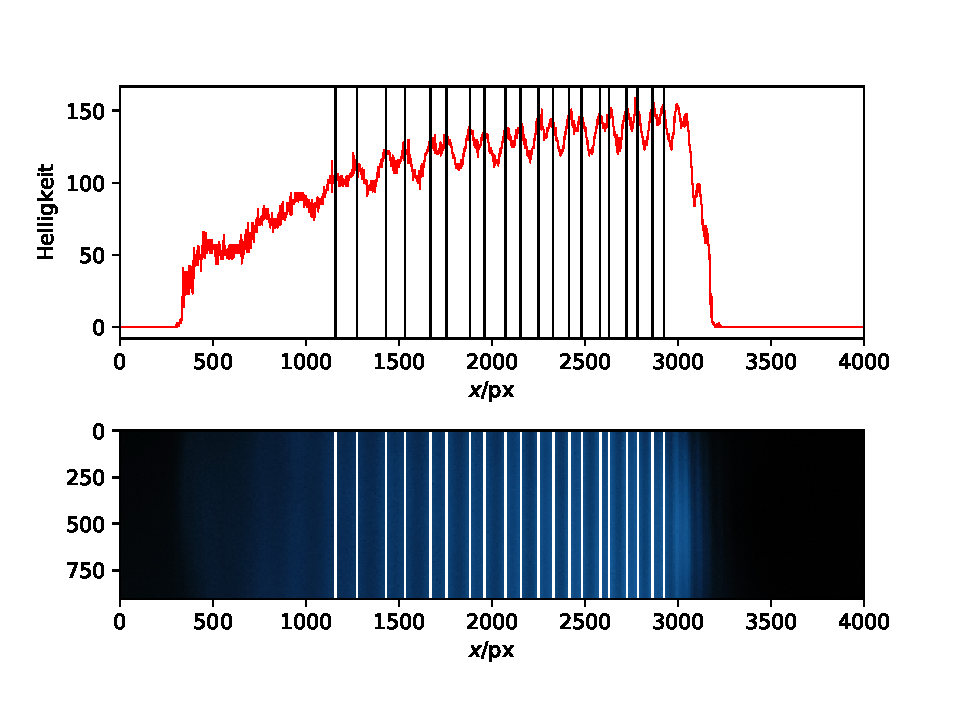
\includegraphics[width = 0.7\textwidth]{../Messdaten/plots/peaks_blau_pi_17.pdf}
  \caption{Blau $\pi$: Darstellung der abgelesenen Lagen der Intesitätsmaxima für das Beugungsbild unter $I =\SI{17}{\ampere}$.}
  \label{fig: peaks_blau_pi_17}
\end{figure}
\input{../Messdaten/tabs/abstände_blau_pi.tex}

